\documentclass{article}

% Put % before of what you want disabled

% Select what to do with todonotes:
% \usepackage[disable]{todonotes} % notes not showed
\usepackage[draft]{todonotes}   % notes showed


\usepackage{lmodern}
\usepackage[T1]{fontenc}
\usepackage[spanish,activeacute]{babel}
\usepackage[utf8]{inputenc}
\usepackage{mathtools}
\usepackage[colorlinks=true]{hyperref}
\usepackage{url}
\hypersetup{
    colorlinks=true,
    linkcolor=blue,
    filecolor=magenta,      
    urlcolor=cyan,
}
\usepackage{graphicx}
\title{Diseño de gramática para la codificación semántica de partituras musicales basada en Humdrum}
\author{Jorge Marco Esteve}

\begin{document}
\maketitle

\section{Antecedentes}
\subsection{Representación Musical}
Los códigos musicales han sido utilizado desde sus inicios para facilitar la transcripción de sonidos, desde los neumas
que se representaban el canto en monasterios medievales, al solfeo de música pedagógica del siglo actual. Muchos códigos
musicales son de uso común, particularmente en la música pedagógica, solfeo. El cual su propósito principal es
inculcar en la mente del cantante la manera de relacionar cada tono con sus vecinos y, por lo tanto,
proporcionar una base sólida para cantar con precisión a simple vista.

Los número de los dedos en piano, los ideogramas los cuales denominamos tablaturas para guitarra y otros instrumentos con trastes,
las notas de notación moderna y muchos símbolos especiales diseñados para transmitir formas particulares de tocar la batería
son códigos de un tipo u otro. En este ámbito, el  código de lenguaje más utilizado y completo para representar el sonido
es la notación musical común o notación musical moderna.

La notación musical moderna o común es la piedra angular en pivota la gran mayoría de sistemas de representación musical actual
y de los últimos siglos.

Entre el s.XIV y el s.XX fueron inventaron diferentes códigos con el fin de alcanzar objetivos que historiadores musicales,
himnógrafos y etnomusicólogos. Pero, desde el siglo XX a la actualidad se ha contemplado la creación de notación para
computadores de una manera sólida, ya que debido a su eficiencia y su memoria resulta una oportunidad codiciosa para,
por ejemplo, representar largas obras musicales con tantos atributos como queramos codificar.

\subsection{Optical Music Recognition (OMR)\cite{OMR}}

Estos últimos años, la disponibilidad de grandes colecciones de partituras digitales ha facilitado tanto la práctica
profesional de la música como el acceso del aficionado a fuentes impresas, ya que había dificultadas para poder obtenerlas
en el pasado. Podemos encontrar ejemplos de estas colecciones en diversas páginas web que llegan a almacenar cientos de
miles de partituras como es el caso de IMSLP \url{http://www.imslp.org}. Además, las bibliotecas públicas y privadas
realizan muchos esfuerzos para publicar sus coleciones online como es en el caso de \url{https://drm.ccarh.org}. Sin
embargo, además de esta accesibilidad a contenido musical, las ventajas de tener una imagen digitalizada de cualquier
obra no se limita a la facilidad de copiarlas y distribuirlas, dichas obras  digitalizadas ofrecen una ausencia de
desgaste que el recurso físico no es capaz de ofrecer.

Las grandes posibilidades que las aplicaciones actuales basadas en música pueden ofrecer están restringidas a partituras codificadas
 de una manera simbólica. Este método de transcripción consiste en el que cada objeto de la composición de una partitura
tiene un símbolo que lo representa y que, agrupándolo cada uno de estos símbolos obtenemos un resultado final que en nuestro
caso será una partitura.

El problema de este método es que la transcripción de las partituras se realiza de forma manual. Esto quiere decir que,
al realizarlo de esta manera, requerimos un coste demasiado en elevado, ya que, el tiempo invertido y la cantidad de recursos
a utilizar llega a resultar prohibitivo debido a la cantidad de material a transcribir. Para eliminar estos inconvenientes
deberíamos obtener una manera de poder transcribir automáticamente estos recursos. El llamado Optical Music Recognition
(OMR) se define como la investigación sobre cómo enseñar a las computadoras a leer notación musical, con el fin de poder
exportar su contenido al formato deseado de manera automática, similar a la utilidad de una caja negra. A pesar de las
grandes ventajas que supone su desarrollo, en estos momentos, OMR está a mitad de camino de ser una IA\footnote{Inteligencia Artificial}
totalmente efectiva, ya que existen problemas muy básicos que OMR no llega a controlar con exactitud, como la eliminación de
las líneas del pentagrama, la localización y clasificación de símbolos, o el ensamblaje de notación musical. Sin embargo, los recientes
avances del aprendizaje automático y, específicamente, del aprendizaje profundo, además de resolver estas tareas con facilidad,
también ayuda a replantearlas para enfrentar todo el proceso de una manera más elegante y compacta, evitando ciertas reglas que hacen que los
sistemas se limiten al tipo de entradas al que estan diseñados.

\subsubsection{Representación agnóstica y representacion semántica}
A día de hoy, Machine Learning es un término muy utilizado en informática que consiste, a grosso modo, en la creación de
sistemas que aprendan automáticamente ciertos patrones a partir de ciertos datos de entrada. La elaboración de estos pueden
ser realizados de diferentes maneras, entre ellas estan, bajo representación agnóstica o representación semántica.

La representación agnóstica corresponde a la enseñanza en el que dado unos patrones de entrada obtendremos una respuesta
que nuestro sistema aprenderá. Por otro lado, la representación semántica guía este aprendizaje mediante ciertas reglas
para que nuestro sistema tenga un menor número de errores.

Dado que OMR permite trabajar tanto con representación agnóstica como semántica, este trabajo intenta mejorar el resutado
de OMR con una gramática formal de **kern\cite{kern} y **mens\cite{mens}, con la esperanza de poder paliar los problemas
que OMR tiene y obtener mejores resultados a la hora de transcribir partituras.

\subsection{Kern y Mens}
 Actualmente hay varios sistemas de representación musical como puede ser DARMS\cite{darms}, SCORE\cite{score},
EsAC\cite{esac}, Kern\cite{kern}. Estos sistemas de representación han sido usados para
codificar simbólicamente partituras, ya sea para renderizarlas a PDF y obtener escritos de ellas, o para reproducirlas,
obteniendo de dichos símbolos una melodía.

Humdrum\cite{humdrum} es un software creado por David Huron en la década de los 80s. Dicho software es empleado con el fin de obtener
diferentes recursos musicales a nivel computacional. Junto a su tipo de notación, **kern, se puede obtener PDFs de partituras
e incluso se puede reproducir la melodía previamente implementada. Esta notacion, **kern, es una representación secuencial musical de manera vertical
en el que cada columna representa una voz de cada melodía con el fin de representar finalmente una partitura. En esta
representación podemos implementar cualquier tipo de notación moderna occidental además de poder manipular los siguientes apartados:

    \begin{itemize}
        \item El tono: alteraciones musicales, claves, posición de claves, armadura, fórmula de compás
        \item La duración: silencios, puntos, ligaduras, ligados.
        \item Articulaciones y Ornamentos: staccato, tenuto, pizzicato.
    \end{itemize}

Una variante de la representación **kern\cite{kern} es **mens\cite{mens}. Este tipo de representación acoge todo tipo de notación mensural blanca
con muchas coincidencias con **kern a la hora de representarse, ya que este tipo de notación también es vertical y se gestiona
de una forma muy parecida a la de notación moderna.

El defecto que lleva a esta representación a no estar realmente completa es la falta de gramática que es el tema correspondiente
a este trabajo.

\subsection{Gramática}
Una gramática es un conjunto finito de reglas en las que se describen mediante símbolos un lenguaje específico. Teniendo
un símbolo inicial del que obtenemos notos terminales y no terminales en los que los nodos terminales los denominamos tokens y
no heredan de el otros nodos y los no terminales generarán más nodos hasta que llegar al punto de que todos los nodos
obtenidos sean terminales.

La finalidad de este trabajo es crear una gramática lo mayormente competente como para poder, a partir de dichas normas y reglas, representar
cualquier tipo de notación musical de la manera más correcta posible. En este caso, la notación **kern y **mens será la adecuada para la creación
de la gramática.
    Obteniendo la primera gramática que comprende los dos tipos de notación: moderna y mensural.

Para implementar nuestra gramática utilizaremos un analizador sintáctico el cual va obteniendo tokens con la finalidad de
decidir si un conjunto de estos tokens cumplen las leyes de nuestra gramática. Hay dos tipos de analizadores sintacticos:
analizador sintáctico descendente y analizador sintáctico ascendente. El primero parte de una regla inicial y concluye en unos
tokens que son generados por las reglas. Mientras el analizador sintactico ascendente parte de un determinado grupo de tokens con
el fin de llegar a una regla principal. Dicho de otra manera, el analizador sintáctico ascendente construye un
arbol desde sus hojas(nodos terminales) hacia su raíz(nodo inicial), mientras que el analizador sintáctico descendente
construye el arbol desde el nodo raiz hasta sus hojas.

Para saber que tipo de analizador sintáctico vamos a utilizar debemos entender que ventajas e inconvenientes tiene cada
uno y hacer balance de ello. El analizador sintáctico ascendente puede resultar muy eficiente la detección de errores es
más rápida respecto al descendente ya que va generando reglas conforme reconoce tokens hasta llegar al nodo raiz. Además, tiene
un reconocimiento muy rápido, aunque no tanto como el descendente. Por otro lado tenemos el analizador sintáctico descendente.
es el método más rápido de las dos variables que barajamos además de ser más sencillo de implementar que la otra alternativa.

Dado que la complejidad que puede suponer una gramática musical puede ser muy elevada, la decisión más acertada en este
caso sería la creación de un analizador sintáctico descendente porque dispondremos de una gran cantidad de tokens y reglas
para poder abordar la mayor parte de expresiones musicales, al ser tan compleja y densa, también deberemos que sea lo más
rápida posible.

Para implementar nuestro analizador usaremos una herramienta denominada ANTLR4\cite{antlr4}. ANTLR4 es un meta-programa
ya que su utilidad reside la creación de otros programas. Desde una descripción formal de la gramática de un lenguaje,
ANTLR genera un programa en el que si una sentencia de dicho lenguaje está escrita de manera incorrecta, este notificará
que lo escrito previamente no pertenece a este lenguaje.

Además, combinaremos ANTLR4 junto con IntelliJ para facilitar la integraciónes de pruebas en las que corroboraremos la utilidad
de nuestra gramática.

\section{Pruebas de caja negra}
Como hemos mencionado anteriormente, la creación de nuestra gramatica será verificada por medio de integración de pruebas,
en nuestro caso, de caja negra.

Las pruebas de caja negra es una técnica de pruebas de software la cual la funcionalidad se verifica sin tomar en cuenta
la estructura interna del código o detalles de implementación. En este tipo de pruebas es necesario tener un gran entendimiento
del tema que se ha programado ya que probaremos comportamientos que sabemos que deberán pasar en el código implementado.
Estas pruebas son unitarias y estan basadas en la especificación en las que dadas unas entradas debemos obtener unas salidas esperadas.

Dado a que nuestro caso, para realizar nuestra gramatica, hemos creado diferentes pruebas especificas de cada apartado musical
 y con una gramática inicial hemos ido pasando cada prueba y en el momento de no pasar una prueba modificaríamos la gramática
hasta poder pasarla. De esta manera obtenemos una gramática verificada mediante nuestras pruebas en la que comprende todos
los comportamientos que nosotros deseabamos. De esta forma obtenemos lo que denominamos un desarrollo guiado por pruebas.

\section{Banco de ejemplos}
\subsection{SKERN}
\subsubsection{Accidentes}
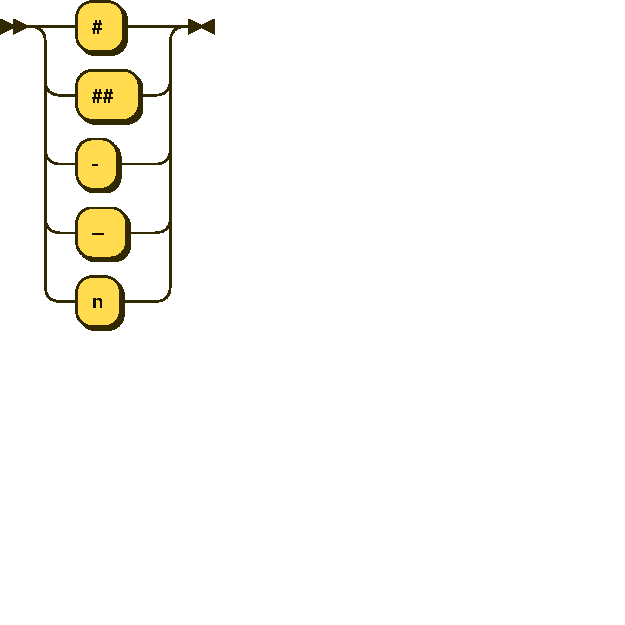
\includegraphics[scale=0.5]{figures_railroad/pdf/skern/accidents.pdf}

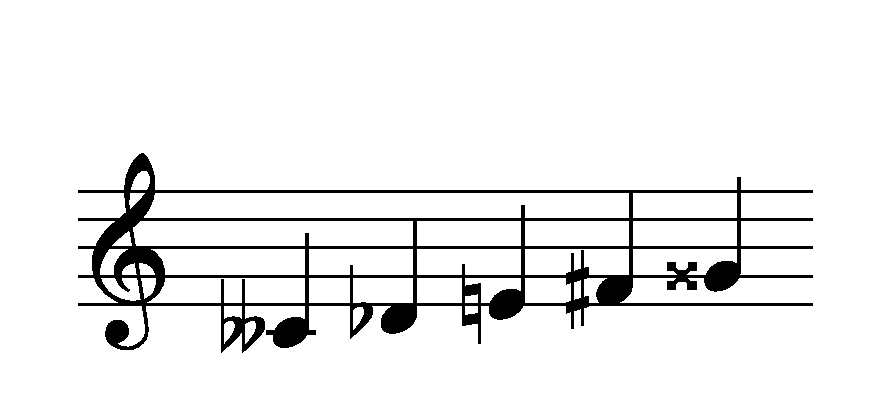
\includegraphics[scale=0.5]{figures_tests/pdf/skern/accident1.pdf}

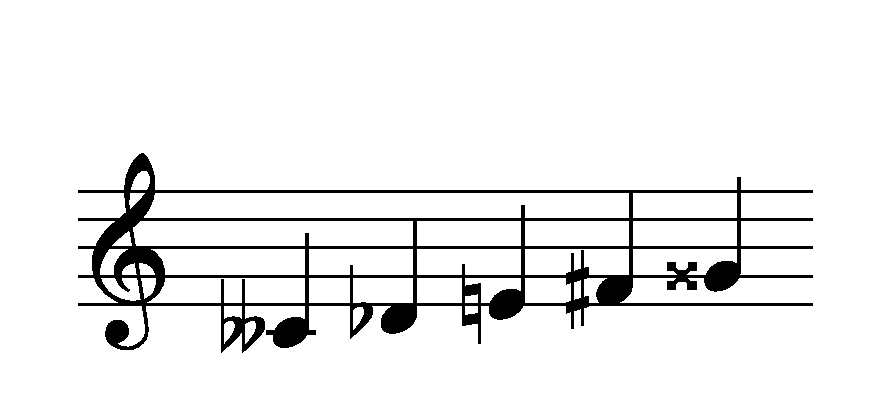
\includegraphics[scale=0.5]{figures_tests/pdf/skern/accident2.pdf}

\subsubsection{Articulationes}
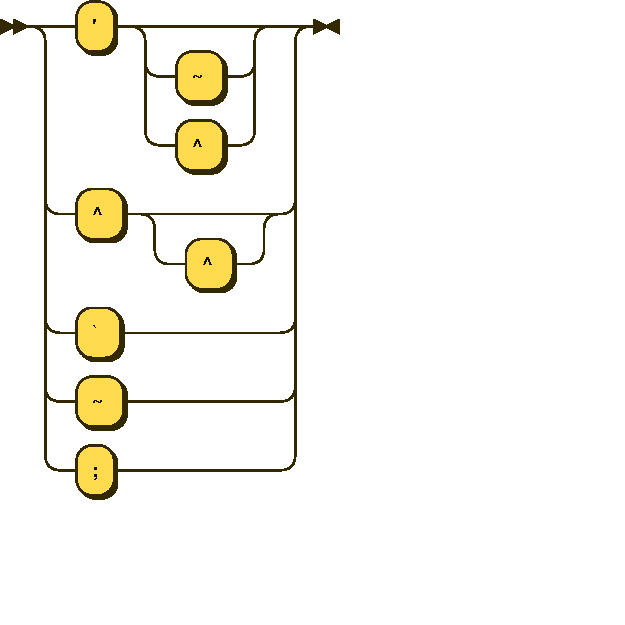
\includegraphics[scale=0.5]{figures_railroad/pdf/skern/articulations.pdf}

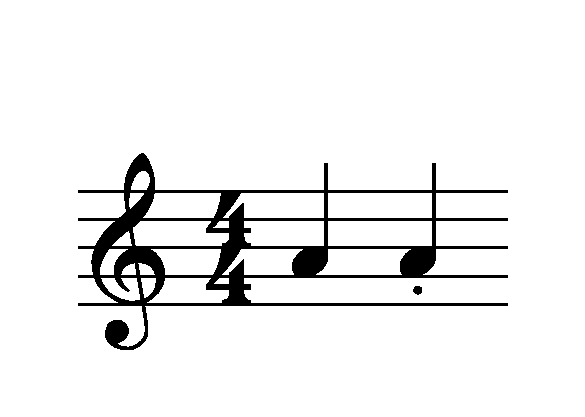
\includegraphics[scale=0.5]{figures_tests/pdf/skern/articulations0.pdf}

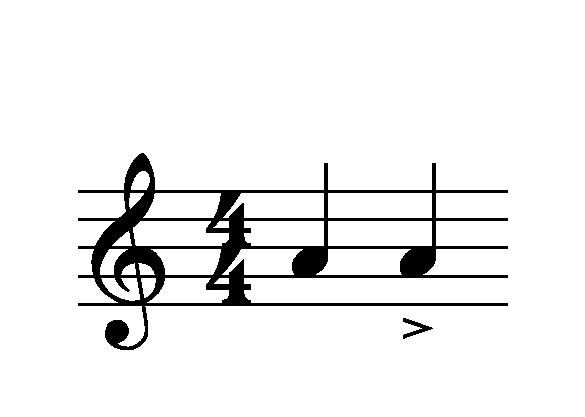
\includegraphics[scale=0.5]{figures_tests/pdf/skern/articulations1.pdf}

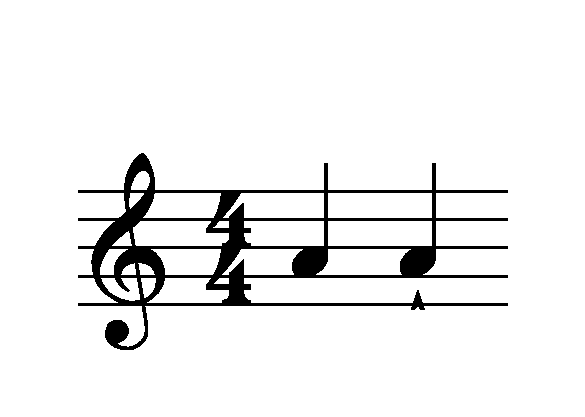
\includegraphics[scale=0.5]{figures_tests/pdf/skern/articulations2.pdf}

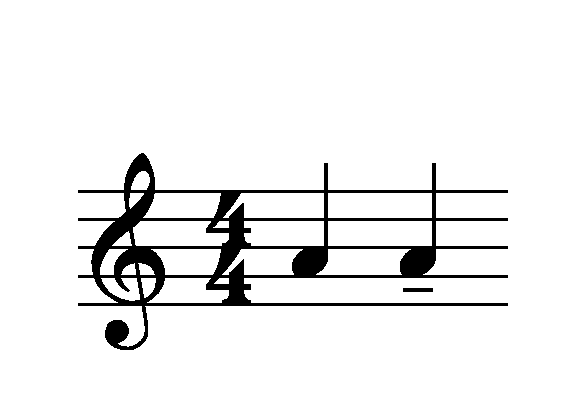
\includegraphics[scale=0.5]{figures_tests/pdf/skern/articulations3.pdf}

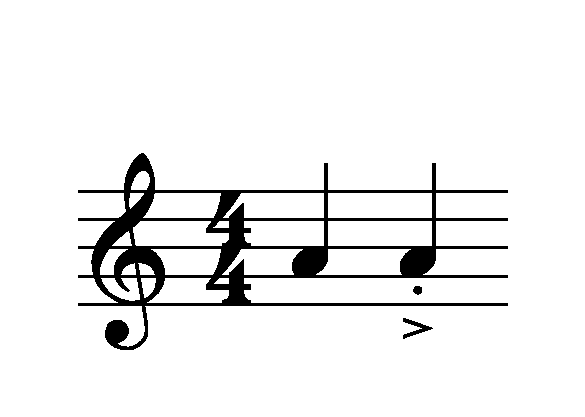
\includegraphics[scale=0.5]{figures_tests/pdf/skern/articulations4.pdf}

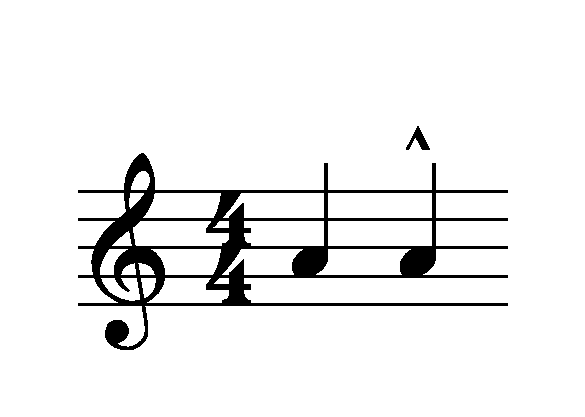
\includegraphics[scale=0.5]{figures_tests/pdf/skern/articulations5.pdf}

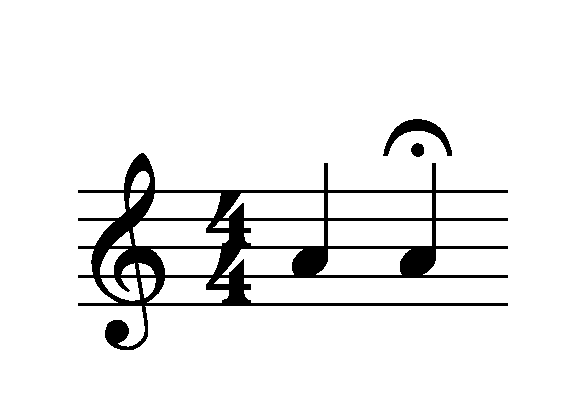
\includegraphics[scale=0.5]{figures_tests/pdf/skern/articulations6.pdf}

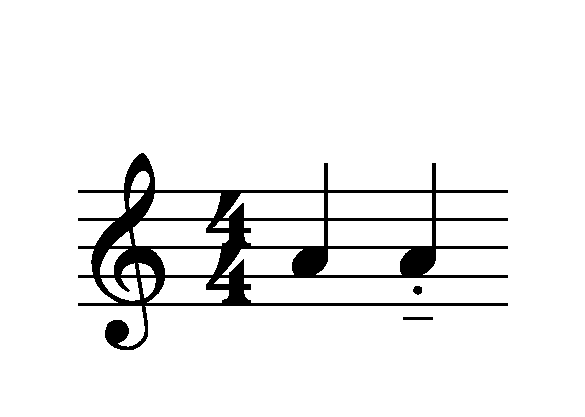
\includegraphics[scale=0.5]{figures_tests/pdf/skern/articulations7.pdf}


\subsubsection{Puntillo}

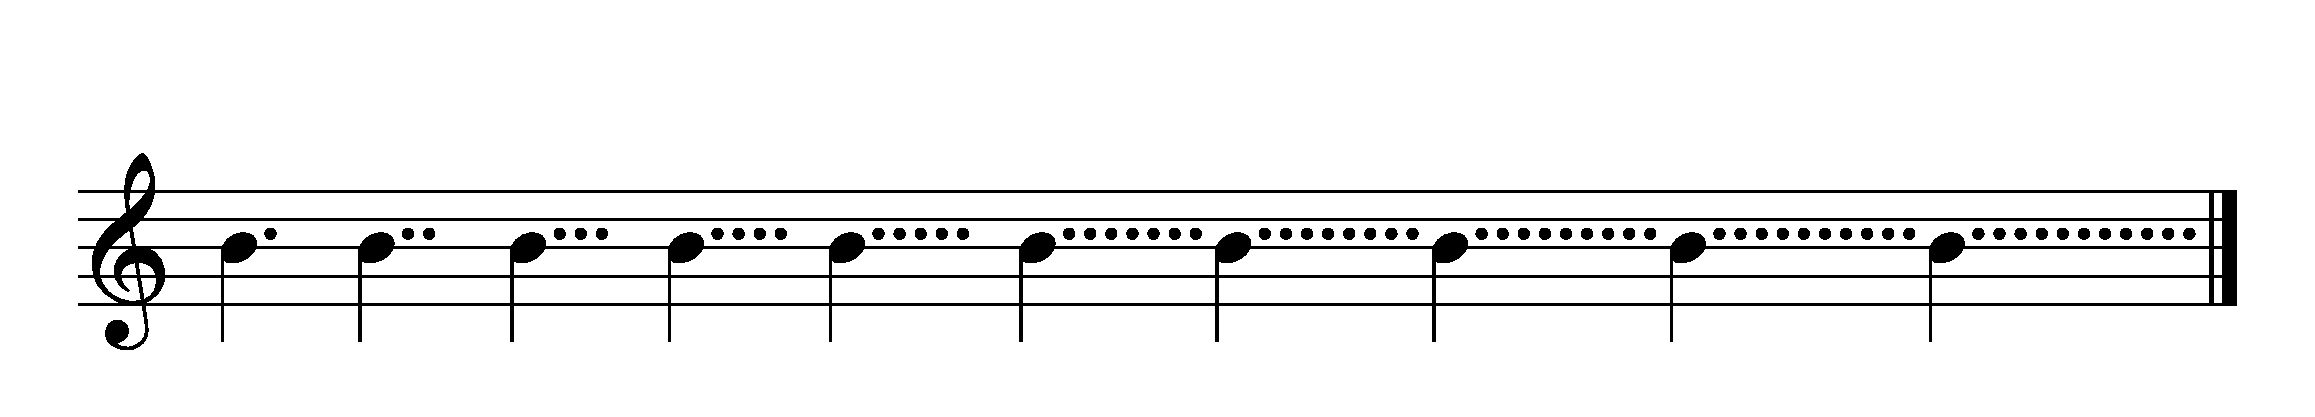
\includegraphics[scale=0.35]{figures_tests/pdf/skern/augmentationDots.pdf}


\subsubsection{Barra de compás}

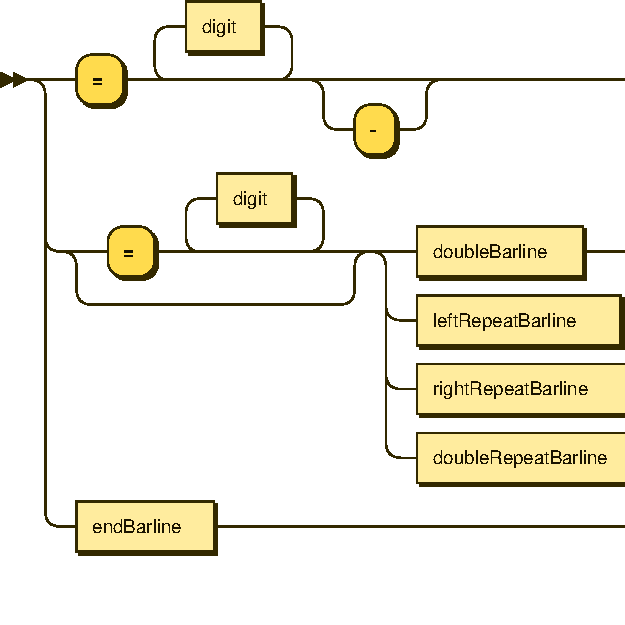
\includegraphics[scale=0.5]{figures_railroad/pdf/skern/barlines.pdf}

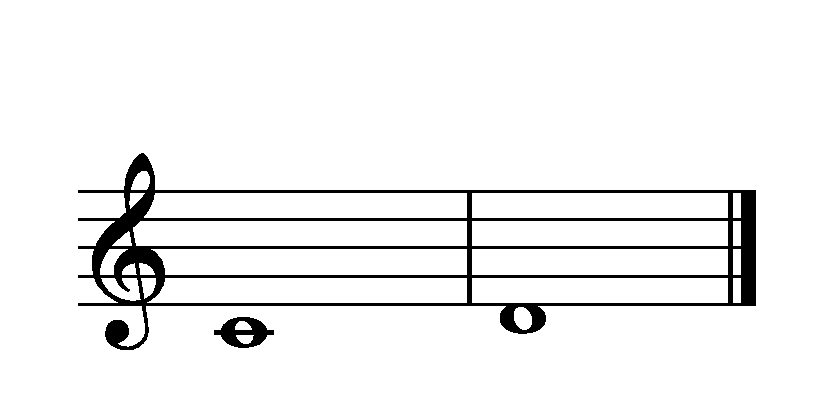
\includegraphics[scale=0.5]{figures_tests/pdf/skern/barlines.pdf}

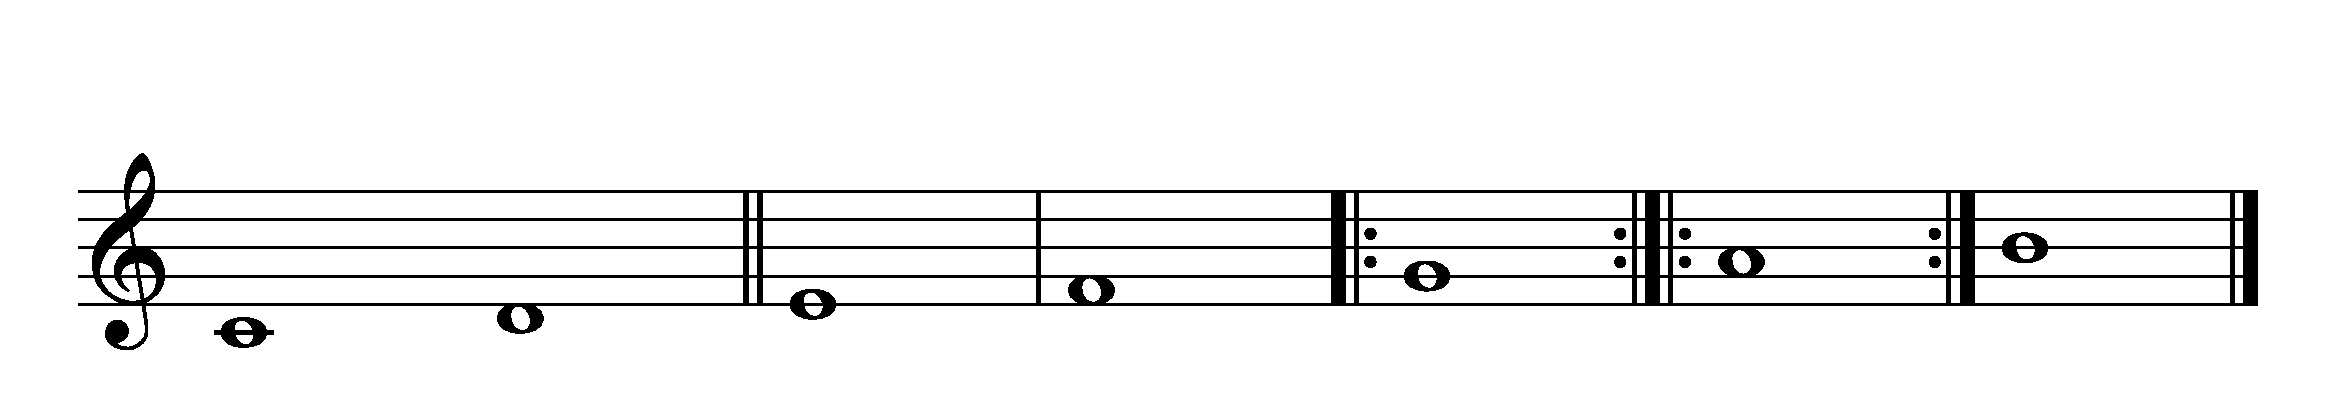
\includegraphics[scale=0.35]{figures_tests/pdf/skern/barlines2.pdf}


\subsubsection{Corcheas}


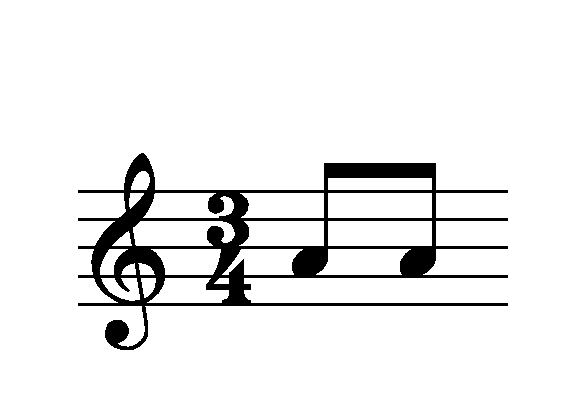
\includegraphics[scale=0.5]{figures_tests/pdf/skern/beaming0.pdf}

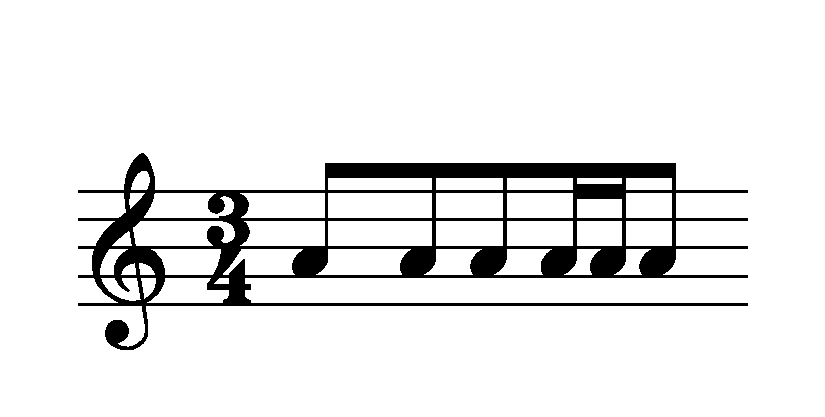
\includegraphics[scale=0.5]{figures_tests/pdf/skern/beaming1.pdf}

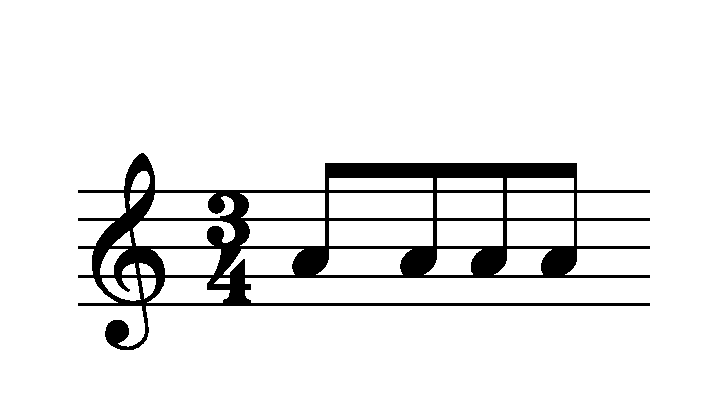
\includegraphics[scale=0.5]{figures_tests/pdf/skern/beaming2.pdf}

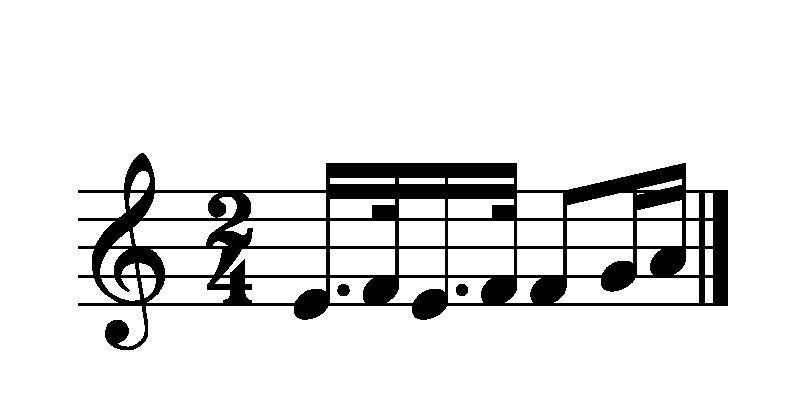
\includegraphics[scale=0.5]{figures_tests/pdf/skern/partialbeaming0.pdf}


\subsubsection{Meter}


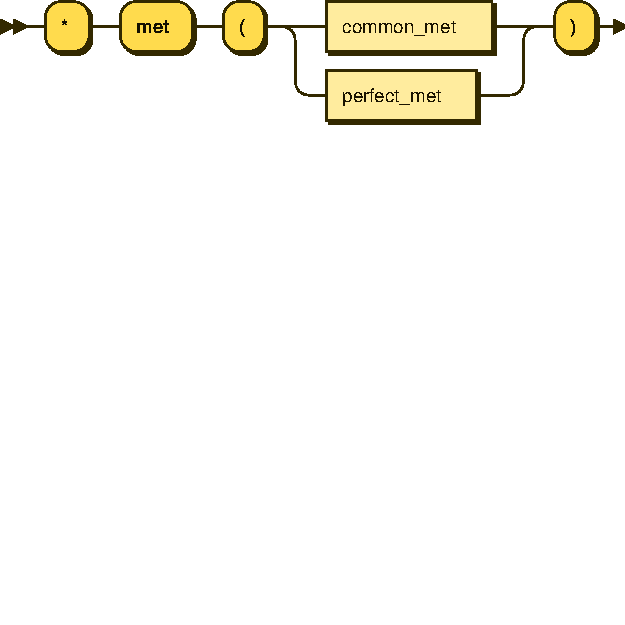
\includegraphics[scale=0.5]{figures_railroad/pdf/skern/meter.pdf}

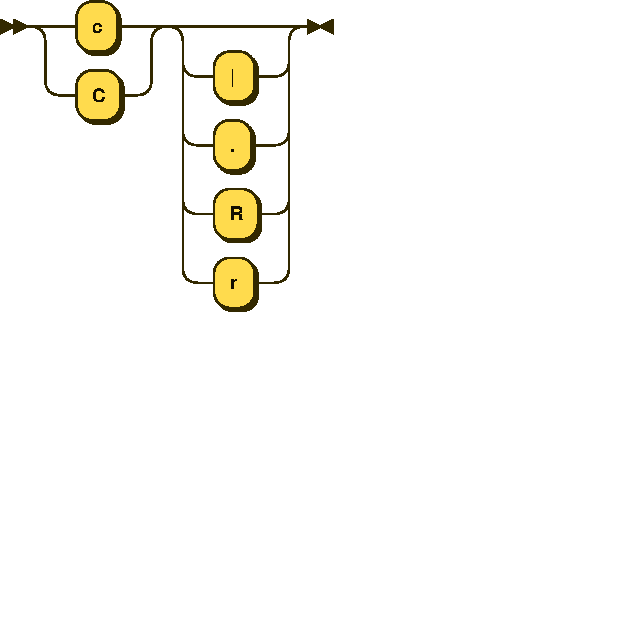
\includegraphics[scale=0.5]{figures_railroad/pdf/skern/commonMeter.pdf}

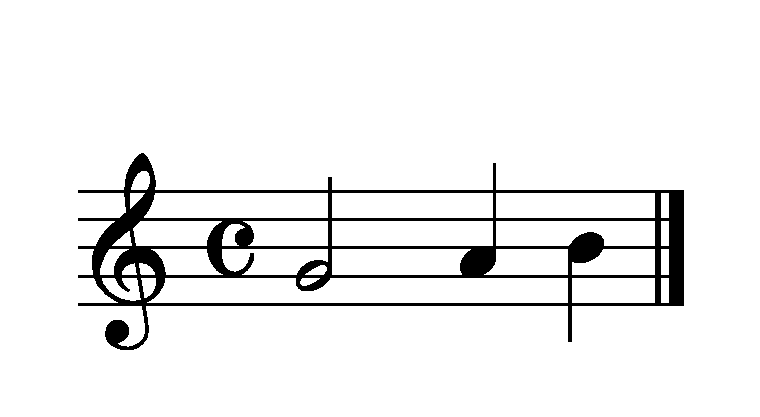
\includegraphics[scale=0.5]{figures_tests/pdf/skern/commonmeter1.pdf}

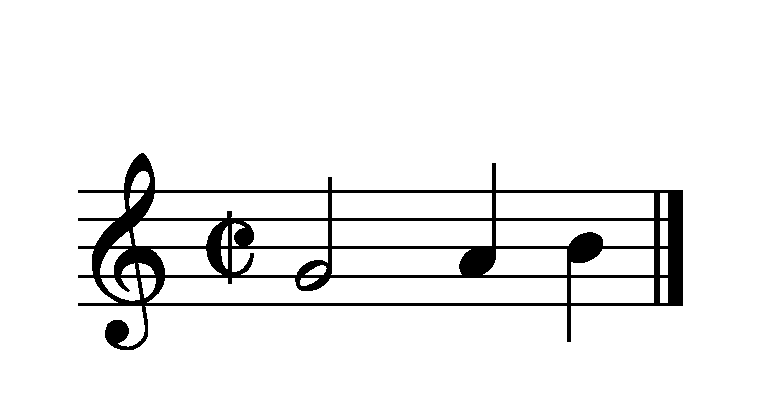
\includegraphics[scale=0.5]{figures_tests/pdf/skern/commonmeter2.pdf}

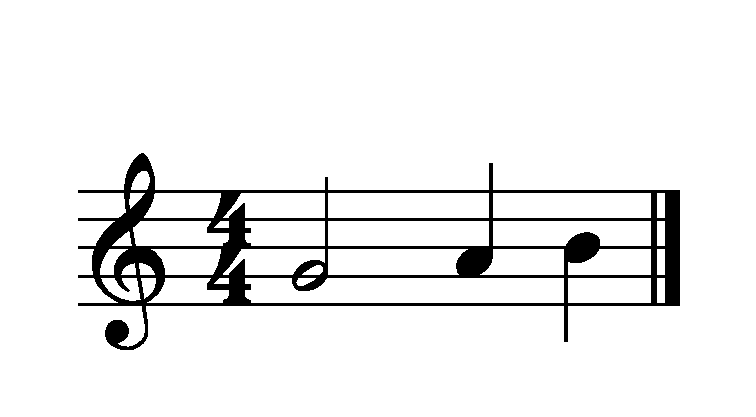
\includegraphics[scale=0.5]{figures_tests/pdf/skern/commonmeter3.pdf}

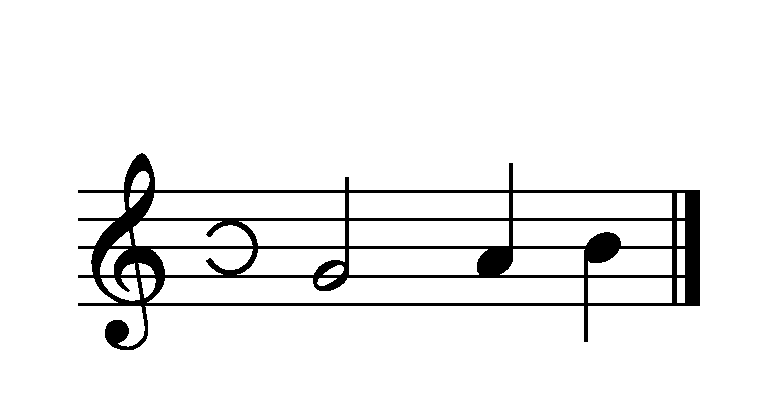
\includegraphics[scale=0.5]{figures_tests/pdf/skern/commonmeter4.pdf}


\subsubsection{Armadura}

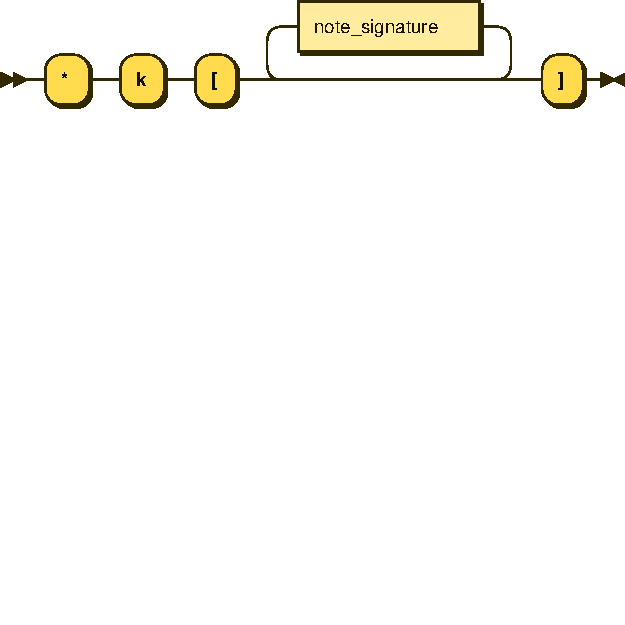
\includegraphics[scale=0.5]{figures_railroad/pdf/skern/keysignature.pdf}
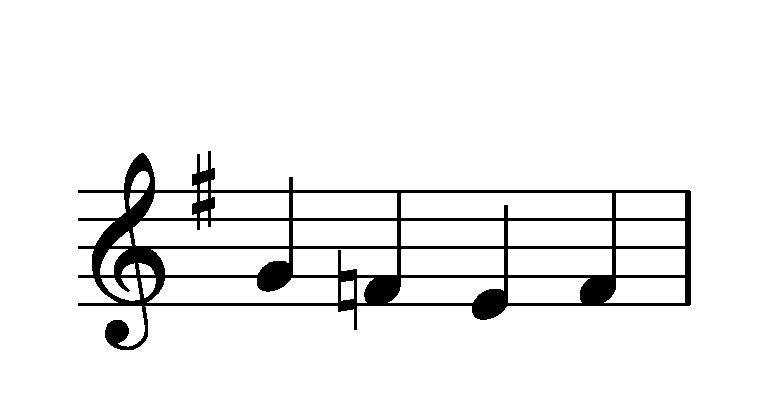
\includegraphics[scale=0.5]{figures_tests/pdf/skern/keysignature1.pdf}

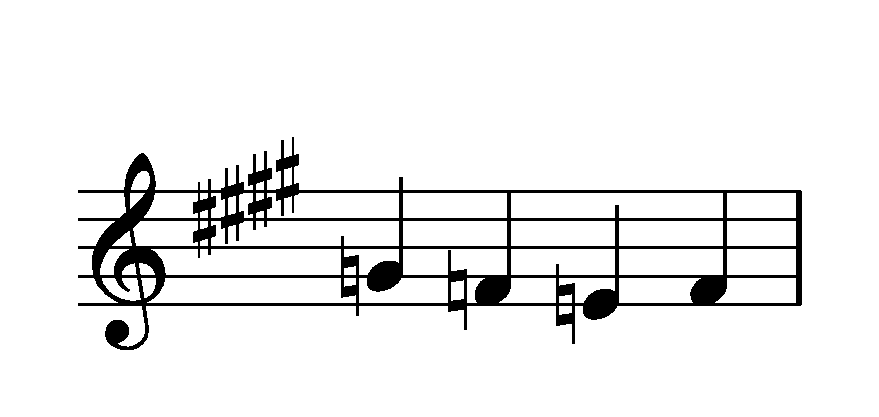
\includegraphics[scale=0.5]{figures_tests/pdf/skern/keysignature2.pdf}

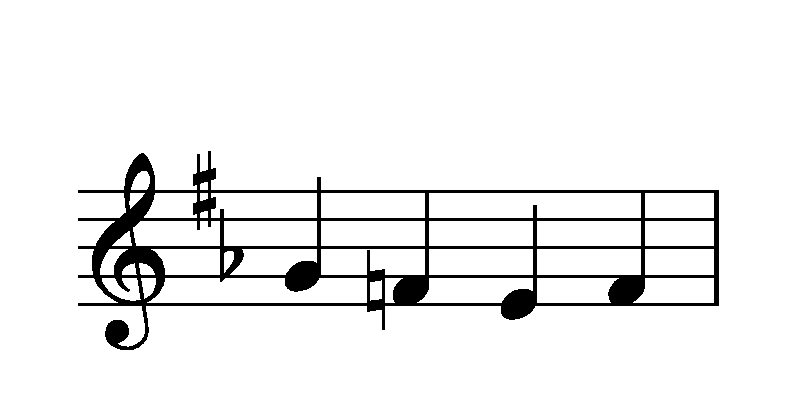
\includegraphics[scale=0.5]{figures_tests/pdf/skern/keysignature3.pdf}

\subsubsection{Notas}

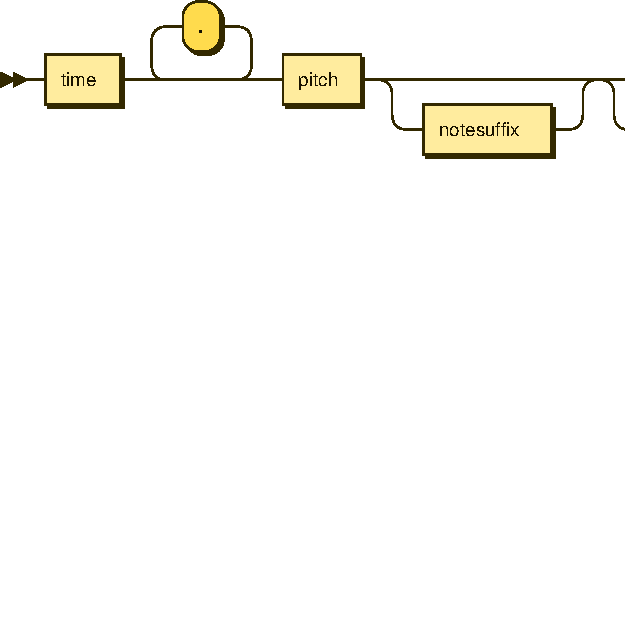
\includegraphics[scale=0.5]{figures_railroad/pdf/skern/notes.pdf}
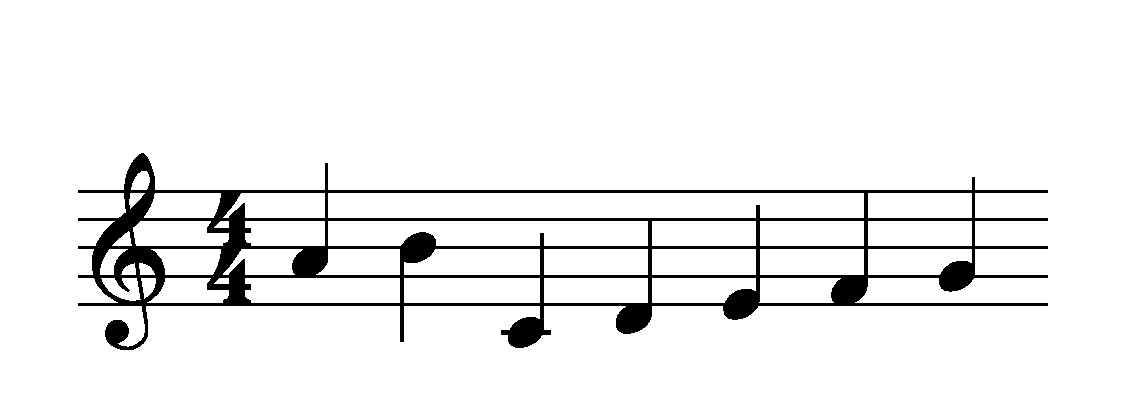
\includegraphics[scale=0.5]{figures_tests/pdf/skern/notename.pdf}

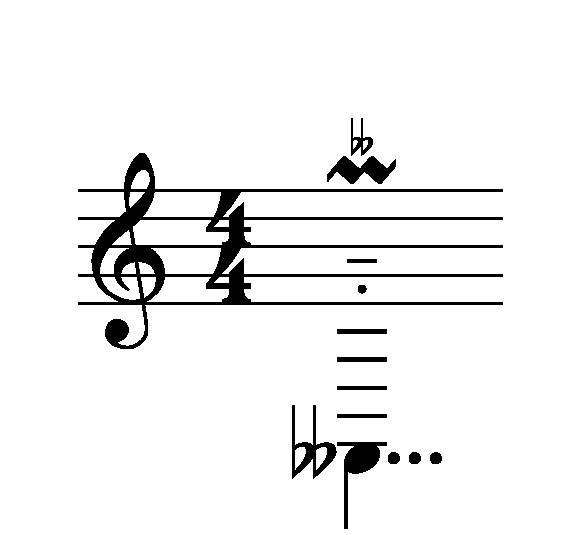
\includegraphics[scale=0.5]{figures_tests/pdf/skern/notesFullAdds.pdf}

\subsubsection{Ornamentos}

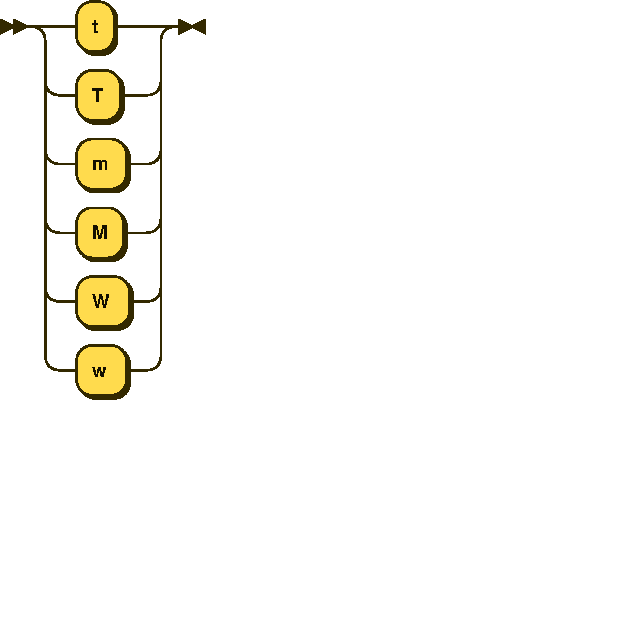
\includegraphics[scale=0.5]{figures_railroad/pdf/skern/ornaments.pdf}
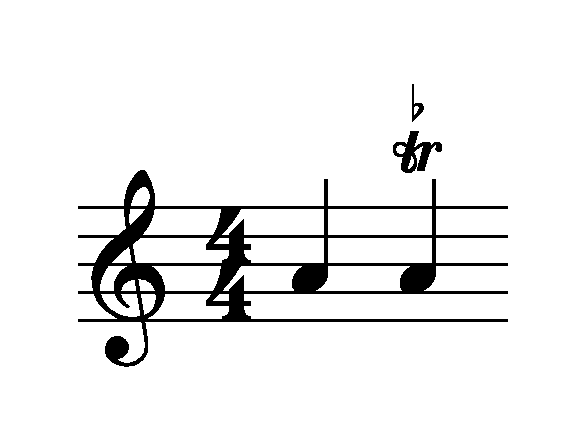
\includegraphics[scale=0.5]{figures_tests/pdf/skern/ornaments0.pdf}

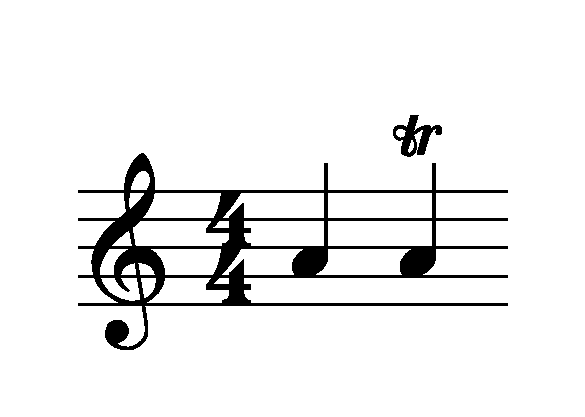
\includegraphics[scale=0.5]{figures_tests/pdf/skern/ornaments1.pdf}

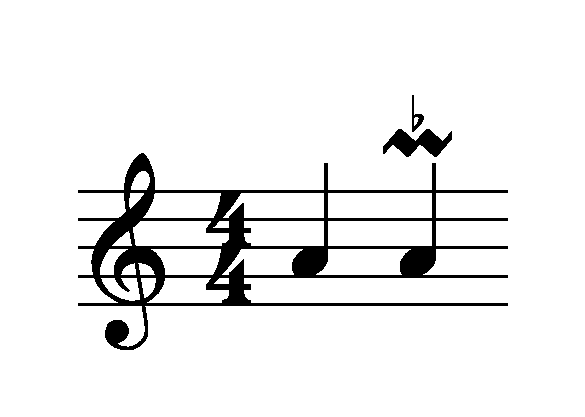
\includegraphics[scale=0.5]{figures_tests/pdf/skern/ornaments2.pdf}

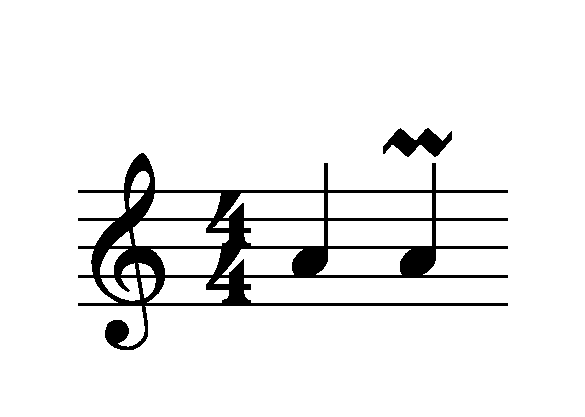
\includegraphics[scale=0.5]{figures_tests/pdf/skern/ornaments3.pdf}

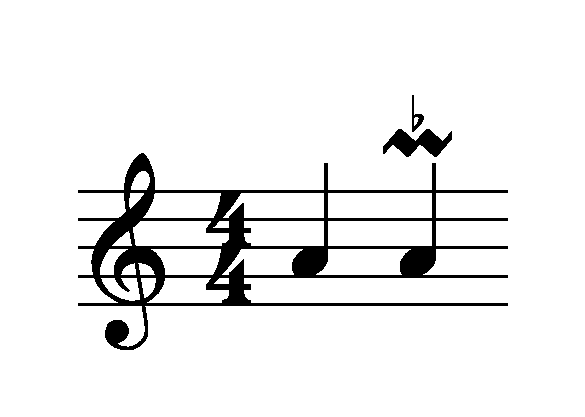
\includegraphics[scale=0.5]{figures_tests/pdf/skern/ornaments4.pdf}

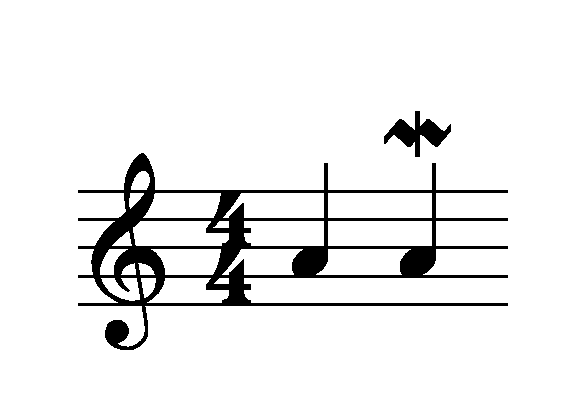
\includegraphics[scale=0.5]{figures_tests/pdf/skern/ornaments5.pdf}

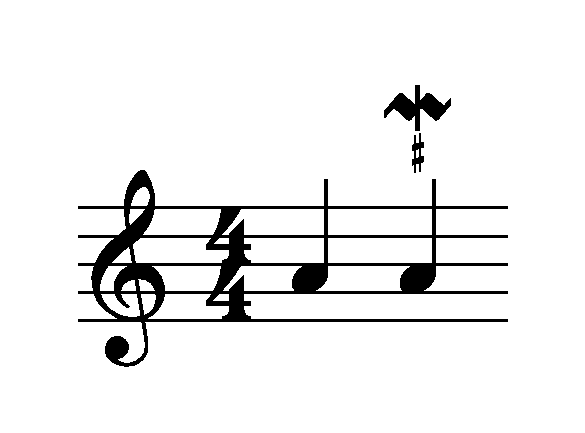
\includegraphics[scale=0.5]{figures_tests/pdf/skern/ornaments6.pdf}

\subsubsection{Silencios}

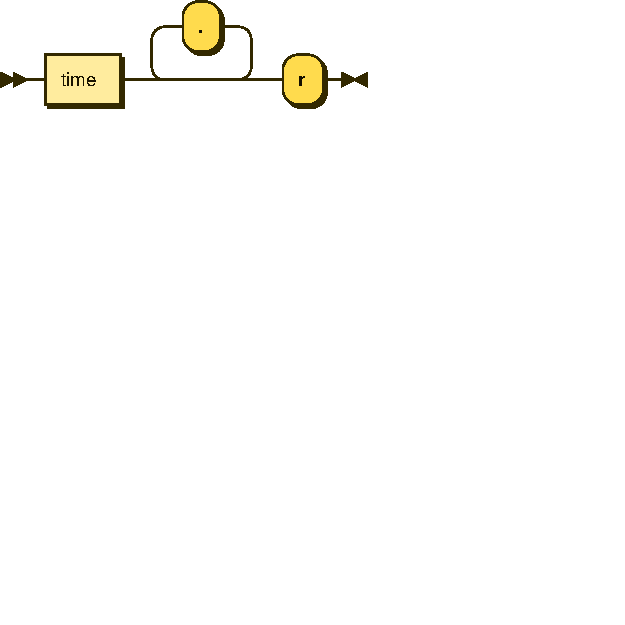
\includegraphics[scale=0.5]{figures_railroad/pdf/skern/rests.pdf}
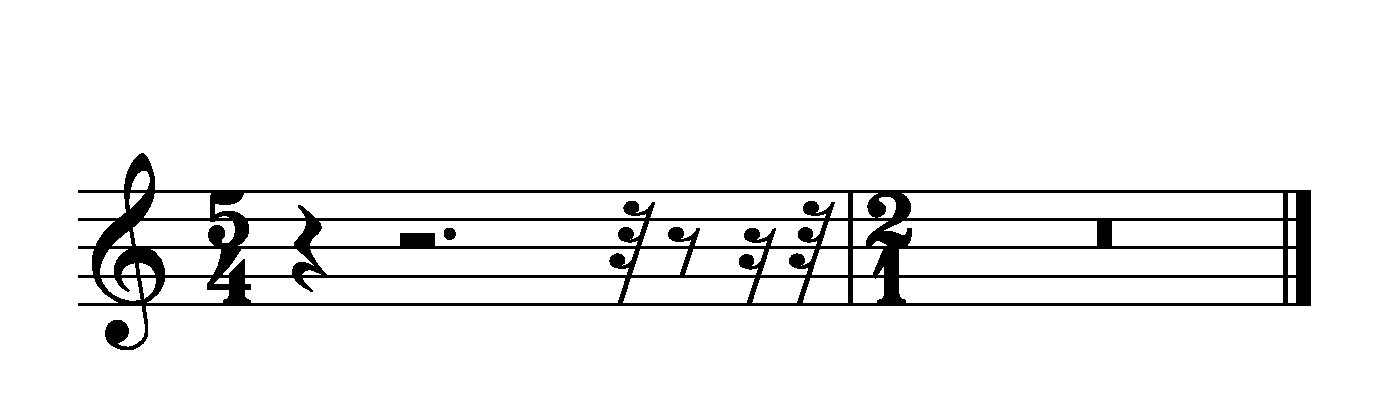
\includegraphics[scale=0.5]{figures_tests/pdf/skern/rest1.pdf}

\subsubsection{Ritmo}

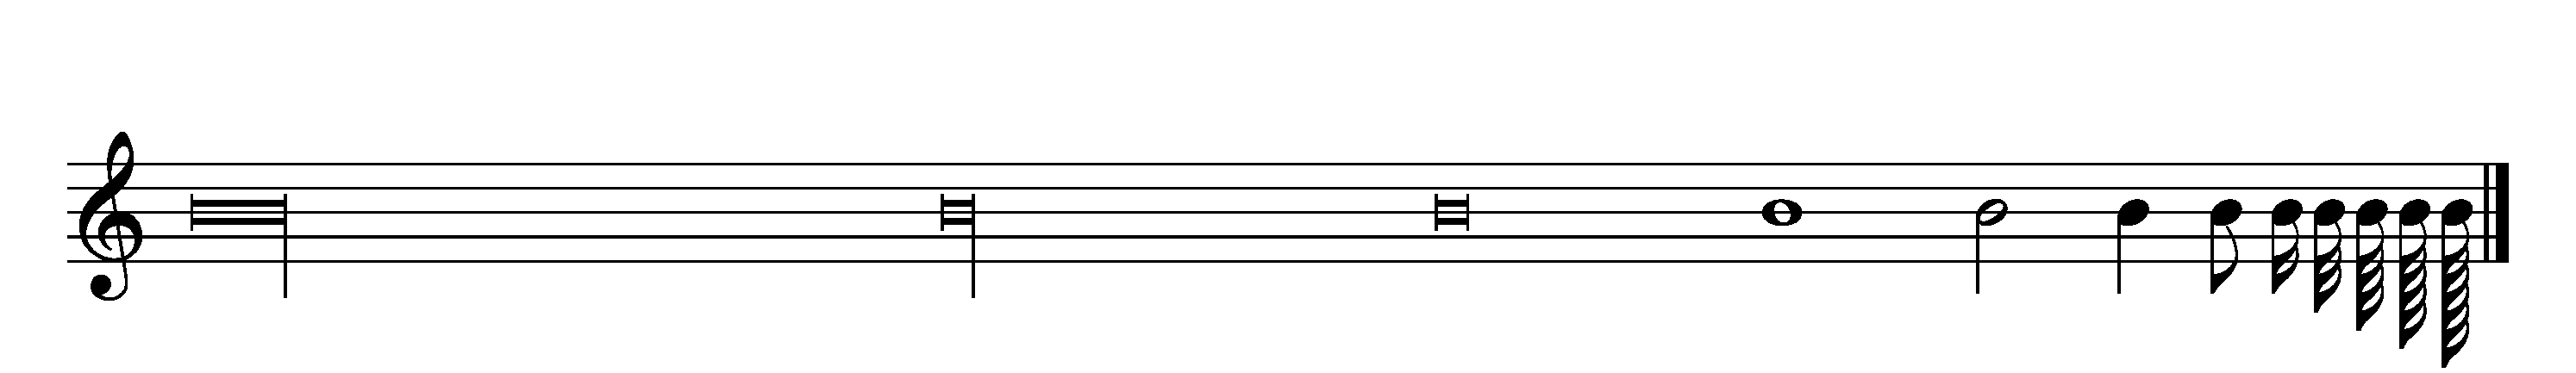
\includegraphics[scale=0.3]{figures_tests/pdf/skern/rhythm.pdf}

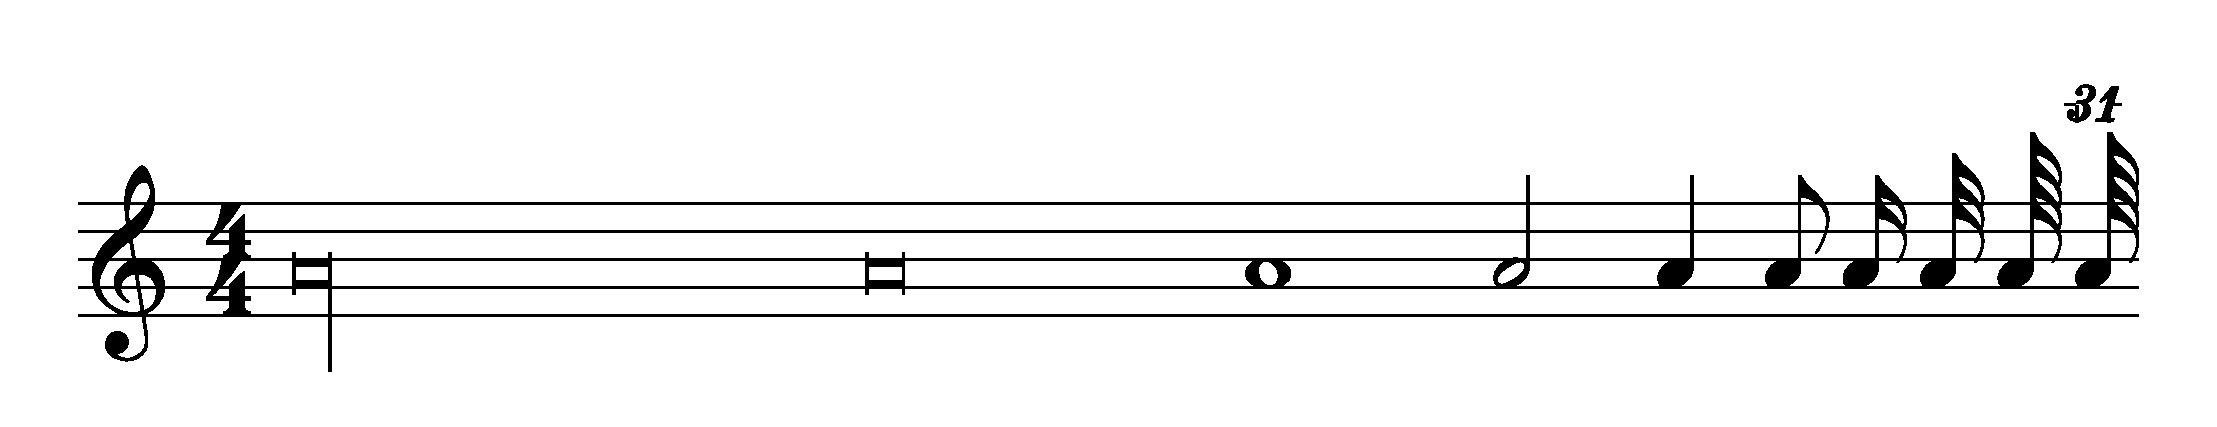
\includegraphics[scale=0.3]{figures_tests/pdf/skern/time.pdf}

\subsubsection{Ligado}

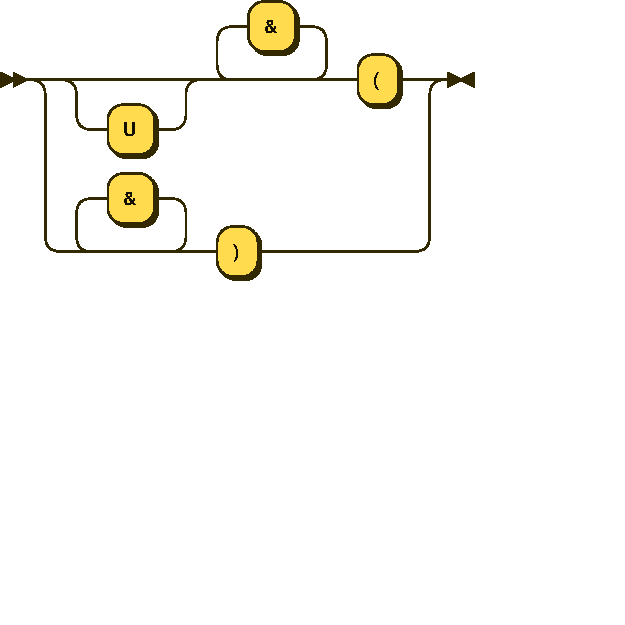
\includegraphics[scale=0.5]{figures_railroad/pdf/skern/slurs.pdf}
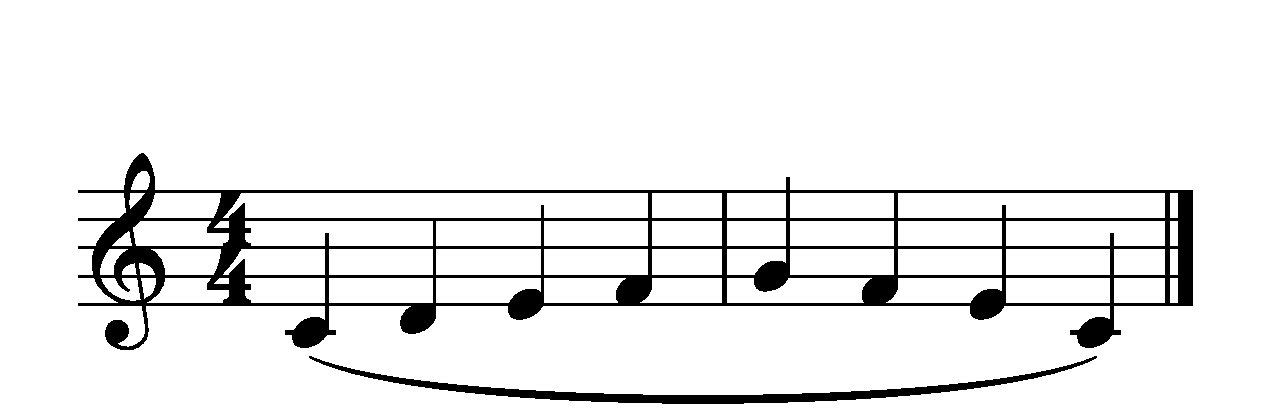
\includegraphics[scale=0.5]{figures_tests/pdf/skern/slur1.pdf}

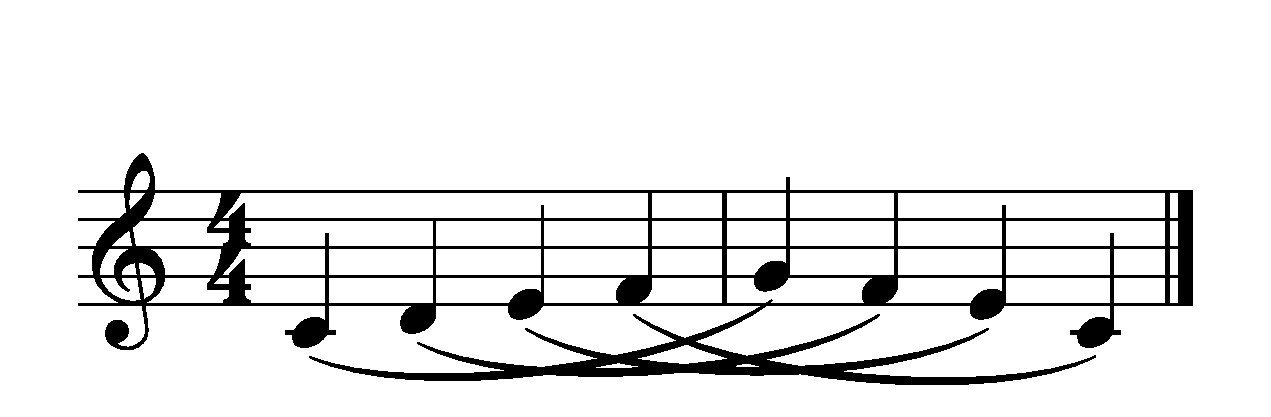
\includegraphics[scale=0.5]{figures_tests/pdf/skern/slur2.pdf}

\subsubsection{Dirección de la plica}

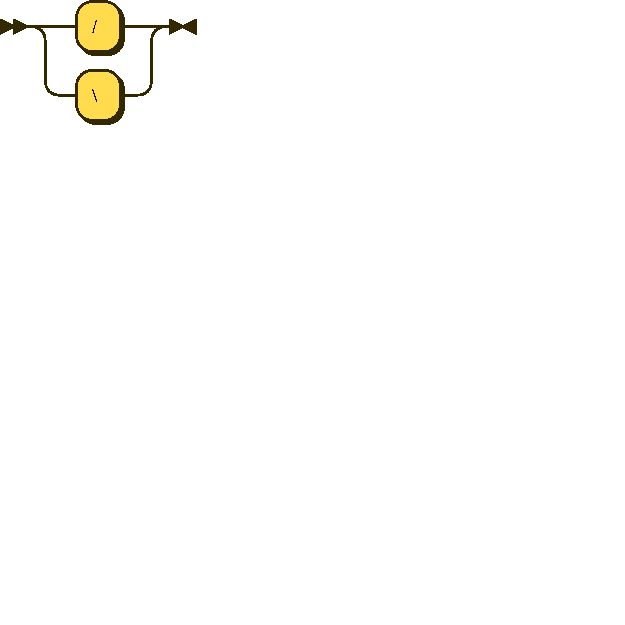
\includegraphics[scale=0.5]{figures_railroad/pdf/skern/stemDirection.pdf}
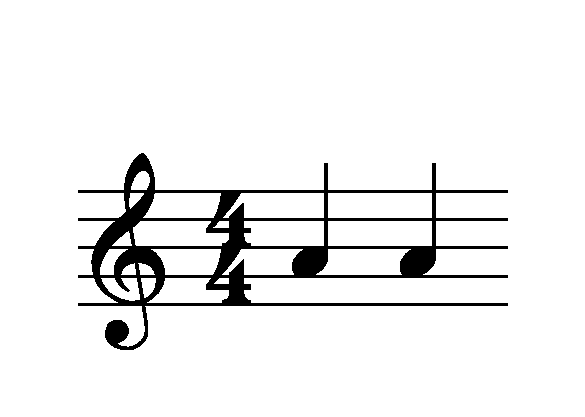
\includegraphics[scale=0.5]{figures_tests/pdf/skern/stemdirection0.pdf}

\includegraphics[scale=0.5]{figures_tests/pdf/skern/stemdirection1.pdf}

\subsubsection{Ligadura}

\includegraphics[scale=0.5]{figures_railroad/pdf/skern/ties.pdf}
\includegraphics[scale=0.5]{figures_tests/pdf/skern/ties1.pdf}

\includegraphics[scale=0.5]{figures_tests/pdf/skern/ties2.pdf}

\includegraphics[scale=0.5]{figures_tests/pdf/skern/ties3.pdf}

\subsubsection{Formula de compas}

\includegraphics[scale=0.5]{figures_railroad/pdf/skern/timesignature.pdf}

\includegraphics[scale=0.5]{figures_tests/pdf/skern/timesignature.pdf}

\includegraphics[scale=0.5]{figures_tests/pdf/skern/timesignature1.pdf}

\includegraphics[scale=0.5]{figures_tests/pdf/skern/timesignature3.pdf}

\subsubsection{Octavas}

\includegraphics[scale=0.5]{figures_railroad/pdf/skern/octaves.pdf}

\includegraphics[scale=0.5]{figures_tests/pdf/skern/octaves.pdf}

\subsubsection{Cambio de configuración}
\includegraphics[scale=0.5]{figures_tests/pdf/skern/changeconfiguration.pdf}

\subsubsection{Acordes}
\includegraphics[scale=0.5]{figures_tests/pdf/skern/chords.pdf}





\subsection{SMENS}
    \subsubsection{Barlines}


        \includegraphics[scale=0.4]{figures_tests/pdf/smens/barlines1.pdf}

    \subsubsection{Dot}
        \includegraphics[scale=0.5]{figures_tests/pdf/smens/dot1.pdf}

    \subsubsection{Ligature}
        \includegraphics[scale=0.5]{figures_tests/pdf/smens/ligature.pdf}

    \subsubsection{Meter}
    \subsubsection*{Common Meter}
        \includegraphics[scale=0.5]{figures_tests/pdf/smens/commonmeter1.pdf}

        \includegraphics[scale=0.5]{figures_tests/pdf/smens/commonmeter2.pdf}

        \includegraphics[scale=0.5]{figures_tests/pdf/smens/commonmeter3.pdf}

        \includegraphics[scale=0.5]{figures_tests/pdf/smens/commonmeter4.pdf}

        \includegraphics[scale=0.5]{figures_tests/pdf/smens/commonmeter5.pdf}

        \includegraphics[scale=0.5]{figures_tests/pdf/smens/commonmeter6.pdf}

        \includegraphics[scale=0.5]{figures_tests/pdf/smens/commonmeter8.pdf}

        \includegraphics[scale=0.5]{figures_tests/pdf/smens/commonmeter9.pdf}

        \includegraphics[scale=0.5]{figures_tests/pdf/smens/commonmeter10.pdf}

        \includegraphics[scale=0.5]{figures_tests/pdf/smens/commonmeter11.pdf}

        \includegraphics[scale=0.5]{figures_tests/pdf/smens/commonmeter12.pdf}

    \subsubsection*{Perfect Meter}
        \includegraphics[scale=0.5]{figures_tests/pdf/smens/perfectmeter1.pdf}

        \includegraphics[scale=0.5]{figures_tests/pdf/smens/perfectmeter2.pdf}

        \includegraphics[scale=0.5]{figures_tests/pdf/smens/perfectmeter3.pdf}

        \includegraphics[scale=0.5]{figures_tests/pdf/smens/perfectmeter4.pdf}

        \includegraphics[scale=0.5]{figures_tests/pdf/smens/perfectmeter5.pdf}

        \includegraphics[scale=0.5]{figures_tests/pdf/smens/perfectmeter6.pdf}

        \includegraphics[scale=0.5]{figures_tests/pdf/smens/perfectmeter7.pdf}

        \includegraphics[scale=0.5]{figures_tests/pdf/smens/perfectmeter8.pdf}

        \includegraphics[scale=0.5]{figures_tests/pdf/smens/perfectmeter9.pdf}

        \includegraphics[scale=0.5]{figures_tests/pdf/smens/perfectmeter10.pdf}

    \subsubsection{Notes}
        \includegraphics[scale=0.5]{figures_tests/pdf/smens/note1.pdf}

    \subsubsection{Note Suffix}
        \includegraphics[scale=0.28]{figures_tests/pdf/smens/notesufix.pdf}

    \subsubsection{Rest}
        \includegraphics[scale=0.3]{figures_tests/pdf/smens/rest1.pdf}

    \subsubsection{Rhythm}
        \includegraphics[scale=0.3]{figures_tests/pdf/smens/rhythm1.pdf}

    \subsubsection{slurs}
        \includegraphics[scale=0.6]{figures_tests/pdf/smens/slur1.pdf}


        \includegraphics[scale=0.6]{figures_tests/pdf/smens/slur2.pdf}

        \todo{Cuidado, las ligaduras / slurs se usan poco en mensural, mejor un ejemplo de notación mdoerna}

    \todo{Los títulos de las secciones en español}

\medskip

\begin{thebibliography}{9}
    \bibitem{OMR}
    Jorge Calvo Zaragoza, David Rizo (2018). End-to-End Neural Optical Music Recognition of Monophonic Scores, Applied Sciences, 6, 606. doi:10.3390/app8040606

    \bibitem{kern}
    Notación musical creada por David Huron en la decada de 1980.
    \texttt{https://www.humdrum.org/guide/ch02/}

    \bibitem{mens}
    Notación mensural blanca derivada de **kern
    \texttt{https://doc.verovio.humdrum.org/humdrum/mens/}

    \bibitem{darms}
    Digital Alternate Representation of Musical Scores creado en 1966 por Stefan Bauer-Mengelberg.

    \bibitem{score}
    Sistema de representación musical creado en 1971 por Leland Smith.

    \bibitem{esac}
    Sistema de representación desarrollado para crear música monofónica a finales de los 80s por Helmut Schaffrasth.

    \bibitem{humdrum}
    \texttt{https://www.humdrum.org}.

    \bibitem{antlr4}
    Terrence Par (2012), \textit{The Definitive ANTLR 4 Reference}. The Pragmatic Programmers, LLC.



\end{thebibliography}

\end{document}
